\documentclass[12pt, letterpaper]{article}

\usepackage[utf8]{inputenc}
\usepackage[spanish]{babel}
\usepackage[margin=2.5cm]{geometry}
\usepackage{graphicx}
\usepackage{booktabs}
\usepackage{longtable}
\usepackage{hyperref}
\usepackage{listings}
\usepackage{xcolor}
\usepackage{float}
\usepackage{enumitem}
\usepackage{titlesec}
\usepackage{fancyhdr}

\pagestyle{fancy}
\fancyhf{}
\rhead{CI-0141 -- Proyecto 2}
\lhead{ECCI -- UCR}
\rfoot{\thepage}

\lstset{
  basicstyle=\ttfamily\small,
  backgroundcolor=\color{gray!10},
  frame=single,
  breaklines=true,
  language=SQL,
  showstringspaces=false
}

\title{
  \textbf{Proyecto Programado 2: ETL y Visualización de Datos} \\[0.5cm]
  \large CI-0141 Bases de Datos Avanzadas \\
  Universidad de Costa Rica \\
  Escuela de Ciencias de la Computación e Informática
}
\author{
  Katherine Acosta Barquero -- B70047 \\
  Elizabeth Huang Wu -- C23913 \\
  Henoc Rojas Carrillo -- C26764 \\
  Christopher Zúñiga Rojas -- C28730
}
\date{Junio 2026}

\begin{document}

\maketitle
\newpage
\tableofcontents
\newpage

% ===========================================================================
\section{Introducción}
% ===========================================================================

Este documento presenta la documentación técnica del Proyecto Programado 2 del curso CI-0141 Bases de Datos Avanzadas. El proyecto consiste en el diseño e implementación de un proceso ETL completo que integra datos de la Escuela de Ciencias de la Computación e Informática (ECCI) de la Universidad de Costa Rica, específicamente las encuestas de ingreso a énfasis aplicadas entre 2021 y 2025.

Los datos se extraen desde tres fuentes en formatos distintos, se transforman y cargan en un Data Warehouse con modelo estrella implementado en PostgreSQL, y se presentan mediante dashboards interactivos en Metabase.

% ===========================================================================
\section{Cliente: Escuela de Ciencias de la Computación e Informática}
% ===========================================================================

\subsection{Descripción del cliente}

La ECCI administra tres énfasis de carrera: Ciencias de la Computación (CC), Ingeniería de Software (IS) e Ingeniería de Tecnologías de la Información (ITI). Cada semestre, los estudiantes de segundo año deben elegir un énfasis, y la escuela aplica encuestas para recopilar información sobre los factores que influyen en esta decisión.

\subsection{Justificación}

Un Data Warehouse que integre los datos históricos de las encuestas de énfasis permite a la ECCI:
\begin{itemize}
  \item Anticipar la demanda de cada énfasis y planificar apertura de grupos.
  \item Identificar qué factores, actividades y canales de comunicación influyen más en la decisión estudiantil.
  \item Evaluar la efectividad de las charlas y actividades organizadas por la escuela.
  \item Detectar patrones de dificultad percibida y correlacionarlos con tasas de reprobación.
  \item Apoyar la asignación de docentes y recursos académicos con datos históricos.
\end{itemize}

% ===========================================================================
\section{Arquitectura del Sistema}
% ===========================================================================

\subsection{Arquitectura general}

El sistema sigue una arquitectura de Data Warehouse clásica con cuatro capas:

\begin{enumerate}
  \item \textbf{Capa de Extracción (Extract):} Conectores para CSV, base de datos relacional PostgreSQL (mock) y API REST (mock JSON).
  \item \textbf{Capa de Transformación (Transform):} Limpieza, normalización, resolución de claves foráneas y generación de dimensiones.
  \item \textbf{Capa de Carga (Load):} Inserción de datos transformados en el modelo dimensional del DW.
  \item \textbf{Capa de Presentación:} Dashboards interactivos en Metabase conectados al DW.
\end{enumerate}

\subsection{Infraestructura}

\begin{table}[H]
\centering
\begin{tabular}{lll}
\toprule
\textbf{Componente} & \textbf{Tecnología} & \textbf{Justificación} \\
\midrule
Data Warehouse & PostgreSQL 16 & Open source, soporte dimensional, extensible \\
ETL & Python 3.11+ (psycopg) & Flexibilidad, ecosistema de datos maduro \\
Visualización & Metabase & Dashboards interactivos, conexión nativa a PG \\
Contenedores & Docker Compose & Reproducibilidad, aislamiento de servicios \\
\bottomrule
\end{tabular}
\caption{Stack tecnológico del proyecto}
\end{table}

\subsection{Diagrama de arquitectura}

\begin{figure}[H]
    \centering
    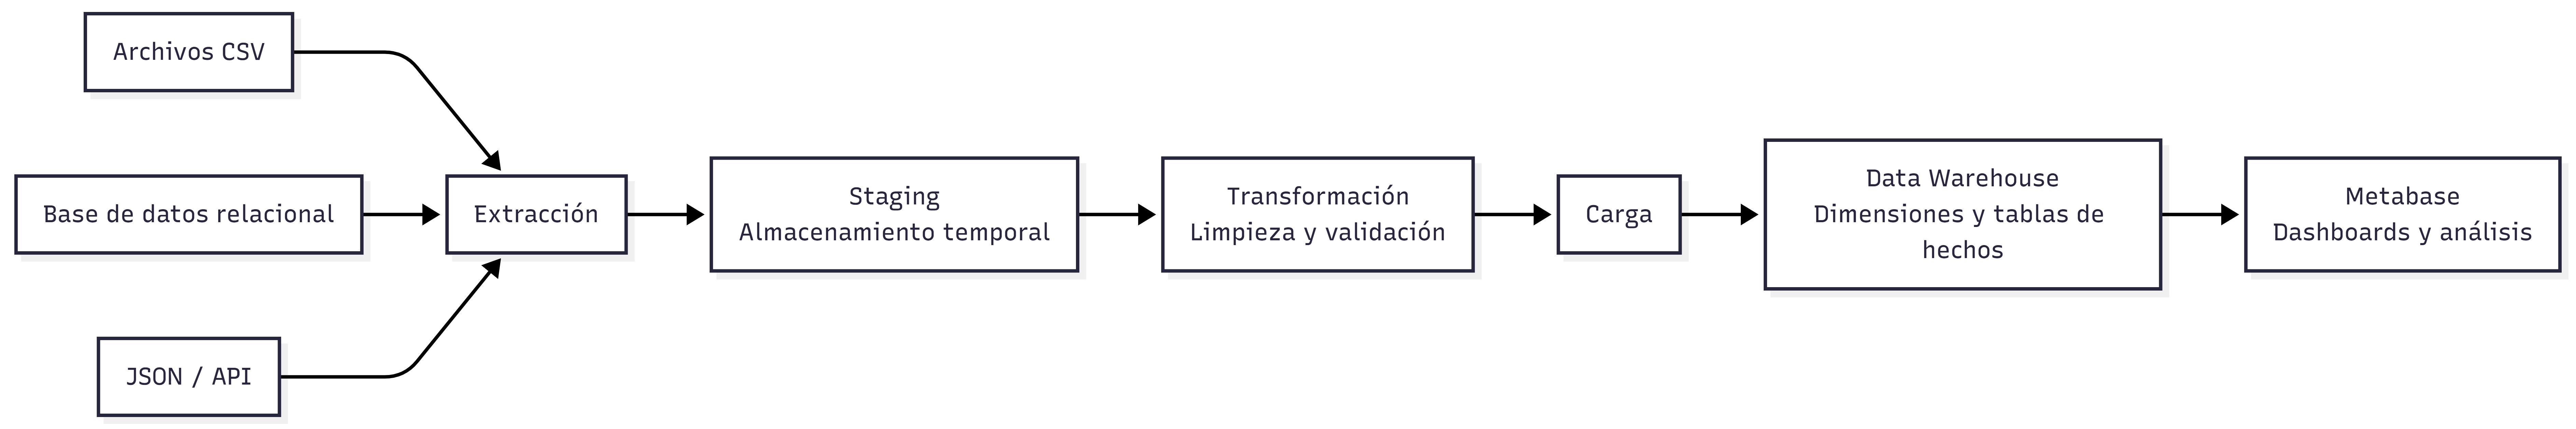
\includegraphics[width=0.95\textwidth]{img/pipeline.png}
    \caption{Arquitectura lógica de la solución}
    \label{fig:arquitectura}
\end{figure}

% ===========================================================================
\section{Fuentes de Datos}
% ===========================================================================

El proyecto integra datos desde tres fuentes con formatos distintos, todas derivadas del mismo dominio (encuestas de énfasis 2021--2025):

\begin{table}[H]
\centering
\begin{tabular}{llp{7cm}}
\toprule
\textbf{Formato} & \textbf{Fuente} & \textbf{Descripción} \\
\midrule
CSV & \texttt{encuesta\_enfasis.csv} & Archivo plano con 269 registros exportados de las encuestas. Contiene todas las columnas del esquema unificado. \\
BD Relacional & \texttt{public.external\_db} & Base de datos PostgreSQL mock con 238 registros. Simula una fuente relacional on-premise. \\
API/JSON & \texttt{encuesta\_enfasis.json} & Archivo JSON con 96 registros. Simula respuesta de una API REST. \\
\bottomrule
\end{tabular}
\caption{Fuentes de datos integradas}
\end{table}

\subsection{Volumen de datos}

Total de registros en staging tras la extracción completa: \textbf{603 registros} (269 + 238 + 96), correspondientes a encuestas de 11 ciclos lectivos (I-2021 a II-2025).

% ===========================================================================
\section{Modelo Dimensional}
% ===========================================================================

\subsection{Esquema estrella}

El Data Warehouse implementa un esquema estrella con una tabla de hechos principal (\texttt{fact\_respuesta}) y múltiples tablas de hechos secundarias para relaciones N:M y calificaciones Likert.

\subsection{Tablas de dimensiones}

\begin{longtable}{llp{6cm}}
\toprule
\textbf{Dimensión} & \textbf{Clave natural} & \textbf{Descripción} \\
\midrule
\endhead
\texttt{dim\_tiempo} & fecha & Año, mes, día, día de semana, trimestre \\
\texttt{dim\_ciclo} & ciclo\_nombre & Ciclo lectivo: I-2021, II-2021, ..., II-2025 \\
\texttt{dim\_enfasis} & codigo & CC, IS, ITI \\
\texttt{dim\_semestre\_carrera} & descripcion & Semestre en que se tomó la decisión \\
\texttt{dim\_canal} & nombre & Canal de comunicación (correo, redes, etc.) \\
\texttt{dim\_factor\_decision} & nombre & Factores que influyeron en la elección \\
\texttt{dim\_actividad} & nombre & Charlas y actividades organizadas \\
\texttt{dim\_bloque\_semestral} & numero\_ciclo & Bloques de cursos (semestres 1--4) \\
\texttt{dim\_area\_conocimiento} & nombre & Áreas/cursos (Programación, Cálculo, etc.) \\
\texttt{dim\_habilidad\_blanda} & nombre & Habilidades blandas evaluadas \\
\texttt{dim\_fuente\_datos} & tipo & Trazabilidad ETL: CSV, BD\_RELACIONAL, API \\
\bottomrule
\caption{Dimensiones del modelo estrella}
\end{longtable}

Todas las dimensiones utilizan claves subrogadas (\texttt{SERIAL PRIMARY KEY}).

\subsection{Tablas de hechos}

\begin{longtable}{lp{8cm}}
\toprule
\textbf{Tabla de hechos} & \textbf{Descripción} \\
\midrule
\endhead
\texttt{fact\_respuesta} & Hecho principal: una fila por encuesta respondida. Contiene métricas de tiempo de respuesta, asistencia, comentarios y FKs a dimensiones. \\
\texttt{fact\_canal\_comunicacion} & Bridge N:M entre respuesta y canales usados. \\
\texttt{fact\_factor\_decision} & Bridge N:M entre respuesta y factores de decisión. \\
\texttt{fact\_calificacion\_actividad} & Impacto y utilidad (Likert 1--5) por actividad. \\
\texttt{fact\_dificultad\_semestre} & Dificultad percibida (Likert 1--5) por bloque semestral. \\
\texttt{fact\_dominio\_conocimiento} & Dominio propio + efectividad de enseñanza por área. \\
\texttt{fact\_habilidad\_blanda} & Mejora percibida en habilidades blandas (1--5). \\
\texttt{fact\_perdida\_curso} & Matriculados y reprobados por ciclo y curso (simulado). \\
\texttt{fact\_auditoria} & Log de cargas ETL: estado, conteos, errores. \\
\bottomrule
\caption{Tablas de hechos del modelo estrella}
\end{longtable}

% ===========================================================================
\section{Diccionario de Datos}
% ===========================================================================

\subsection{staging.encuesta\_enfasis\_raw}

Zona de aterrizaje cruda. Todas las columnas son de tipo \texttt{TEXT} (la normalización ocurre en la capa Transform). Campos principales:

\begin{longtable}{lp{8cm}}
\toprule
\textbf{Columna} & \textbf{Descripción} \\
\midrule
\endhead
\texttt{id\_staging} & PK autoincremental \\
\texttt{id\_fuente} & FK lógica a dim\_fuente\_datos \\
\texttt{archivo\_origen} & Nombre del archivo/fuente de origen \\
\texttt{term} & Ciclo lectivo (``I Ciclo'', ``II Ciclo'') \\
\texttt{year} & Año del ciclo \\
\texttt{response\_id} & ID original de la respuesta \\
\texttt{submitted\_at} & Timestamp de envío \\
\texttt{started\_at} & Timestamp de inicio \\
\texttt{heard\_*} & Canales por los que se enteró (Sí/No) \\
\texttt{attended} & Si asistió a las actividades \\
\texttt{decision\_semester} & Semestre en que tomó la decisión \\
\texttt{factor\_*} & Factores de decisión (Sí/No) \\
\texttt{impact\_*} & Impacto de actividades (categórico/Likert) \\
\texttt{useful\_*} & Utilidad de actividades (Likert 1--5) \\
\texttt{chosen\_emphasis} & Énfasis elegido (CC/IS/ITI) \\
\texttt{difficulty\_cycle\_*} & Dificultad percibida por bloque (1--5) \\
\texttt{axis1\_*/axis2\_*} & Dominio propio / efectividad de enseñanza \\
\texttt{skill\_*} & Mejora en habilidades blandas (1--5) \\
\texttt{time\_*} & Tiempos de respuesta en segundos \\
\bottomrule
\caption{Campos principales de la tabla de staging}
\end{longtable}

\subsection{dw.fact\_respuesta}

\begin{longtable}{llp{6cm}}
\toprule
\textbf{Columna} & \textbf{Tipo} & \textbf{Descripción} \\
\midrule
\endhead
\texttt{id\_respuesta\_sk} & SERIAL PK & Clave subrogada \\
\texttt{id\_respuesta\_src} & INTEGER & ID original del sistema fuente \\
\texttt{id\_ciclo} & INTEGER FK & Referencia a dim\_ciclo \\
\texttt{id\_tiempo\_envio} & INTEGER FK & Fecha de envío \\
\texttt{id\_tiempo\_inicio} & INTEGER FK & Fecha de inicio \\
\texttt{id\_enfasis} & INTEGER FK & Énfasis elegido \\
\texttt{id\_semestre\_decision} & INTEGER FK & Semestre de la decisión \\
\texttt{id\_fuente} & INTEGER FK & Fuente de datos (CSV/BD/API) \\
\texttt{asistio} & BOOLEAN & Asistió a actividades \\
\texttt{influyo\_actividades} & VARCHAR(20) & Sí/No/Parcialmente/N/A \\
\texttt{tiempo\_total\_seg} & NUMERIC(10,2) & Tiempo total de respuesta \\
\texttt{pagina\_alcanzada} & SMALLINT & Última página completada \\
\texttt{fecha\_carga} & TIMESTAMP & Fecha de carga ETL \\
\bottomrule
\caption{Columnas principales de fact\_respuesta}
\end{longtable}

\subsection{dw.fact\_perdida\_curso}

\begin{longtable}{llp{6cm}}
\toprule
\textbf{Columna} & \textbf{Tipo} & \textbf{Descripción} \\
\midrule
\endhead
\texttt{id\_perdida} & SERIAL PK & Clave subrogada \\
\texttt{id\_ciclo} & INTEGER FK & Ciclo lectivo \\
\texttt{id\_area} & INTEGER FK & Curso/área de conocimiento \\
\texttt{matriculados} & INTEGER & Estudiantes matriculados \\
\texttt{reprobados} & INTEGER & Estudiantes que reprobaron \\
\texttt{tasa\_reprobacion} & NUMERIC(5,2) & Calculada: (reprobados/matriculados)*100 \\
\bottomrule
\caption{Columnas de fact\_perdida\_curso (datos simulados)}
\end{longtable}

% ===========================================================================
\section{Proceso ETL}
% ===========================================================================

\subsection{Extracción}

La capa de extracción está implementada en \texttt{etl/extract/} y consta de tres conectores:

\begin{enumerate}
  \item \textbf{CSV (\texttt{csv\_source.py}):} Lee \texttt{preprocessed\_data/encuesta\_enfasis.csv} y carga las filas en \texttt{staging.encuesta\_enfasis\_raw} con \texttt{id\_fuente=1}.
  \item \textbf{BD Relacional (\texttt{relational\_source.py}):} Crea la tabla mock \texttt{public.external\_db} desde un script SQL y extrae a staging con \texttt{id\_fuente=2}.
  \item \textbf{JSON/API (\texttt{json\_source.py}):} Lee \texttt{preprocessed\_data/encuesta\_enfasis.json} y carga a staging con \texttt{id\_fuente=3}.
\end{enumerate}

Todos los extractores son idempotentes: eliminan filas previas de la misma fuente antes de insertar.

\subsection{Transformación}

La capa de transformación (\texttt{etl/transform/}) realiza:

\begin{itemize}
  \item \textbf{Generación de dim\_tiempo:} Extrae fechas únicas de \texttt{submitted\_at} y \texttt{started\_at} en staging e inserta en \texttt{dw.dim\_tiempo}.
  \item \textbf{Normalización:} Parseo de valores Likert en múltiples formatos (``3'', ``Muy fácil: 1'', ``5 - Muy útil''), mapeo Sí/No a booleanos, extracción de códigos de énfasis, construcción de claves naturales de ciclo.
  \item \textbf{Resolución de FKs:} Mapeo de valores textuales a claves subrogadas de las dimensiones.
  \item \textbf{Limpieza:} Tratamiento de valores nulos, N/A, blancos y formatos inconsistentes entre ciclos.
\end{itemize}

\subsection{Carga}

La carga (\texttt{etl/transform/load\_facts.py}) implementa:

\begin{itemize}
  \item \textbf{Estrategia full reload:} Trunca todas las tablas de hechos y reconstruye desde staging en cada ejecución.
  \item \textbf{Manejo de duplicados:} \texttt{ON CONFLICT DO NOTHING} para registros repetidos.
  \item \textbf{Auditoría:} Registra en \texttt{fact\_auditoria} el estado (EXITOSO/FALLIDO), conteos de registros procesados, insertados y rechazados por fuente.
  \item \textbf{Transaccionalidad:} Toda la carga ocurre en una sola transacción; en caso de error se hace rollback y se registra el fallo.
\end{itemize}

\subsection{Orquestación}

El pipeline completo se ejecuta secuencialmente desde \texttt{etl/main.py}:

\begin{lstlisting}[language=bash]
python -m etl.main
\end{lstlisting}

Pasos en orden:
\begin{enumerate}
  \item \texttt{relational\_setup\_mock\_source} -- Crea la BD mock
  \item \texttt{clean\_raw\_staging} -- Vacía staging
  \item \texttt{csv\_to\_raw\_staging} -- Extrae CSV
  \item \texttt{relational\_extract\_to\_staging} -- Extrae BD relacional
  \item \texttt{json\_extract\_to\_staging} -- Extrae JSON
  \item \texttt{transform\_dim\_tiempo} -- Genera dimensión tiempo
  \item \texttt{transform\_load\_facts} -- Carga tablas de hechos
\end{enumerate}

% ===========================================================================
\section{Dashboards}
% ===========================================================================

Los dashboards se implementan en Metabase, conectado directamente al Data Warehouse PostgreSQL. La selección de visualizaciones se basa en los tipos de gráfico que mejor representan la naturaleza de cada conjunto de datos.

\subsection{Dashboard 1: Proyección de Demanda de Énfasis}

\begin{itemize}
  \item \textbf{Objetivo:} Estimación de la demanda futura de cada énfasis a partir de tendencias históricas y patrones de decisión.
  \item \textbf{Datos requeridos:}
  \begin{itemize}
    \item \texttt{chosen\_emphasis} (énfasis elegido)
    \item \texttt{term}, \texttt{year} (ciclo y año)
    \item \texttt{decision\_semester} (semestre en que se tomó la decisión)
    \item Cantidad de personas que reprobaron cursos (datos simulados en \texttt{fact\_perdida\_curso})
  \end{itemize}
  \item \textbf{Tablas del DW:} \texttt{fact\_respuesta}, \texttt{fact\_perdida\_curso}, \texttt{dim\_ciclo}, \texttt{dim\_enfasis}, \texttt{dim\_semestre\_carrera}, \texttt{dim\_area\_conocimiento}.
  \item \textbf{Visualizaciones:}
  \begin{itemize}
    \item Gráfico de línea: evolución de la elección de énfasis por ciclo.
    \item Gráfico de barras agrupadas: tasa de reprobación por curso y ciclo.
    \item KPI: distribución porcentual actual CC/IS/ITI.
    \item Tabla: proyección de matrícula por énfasis para el siguiente ciclo.
  \end{itemize}
  \item \textbf{Toma de decisiones:} Permite anticipar la cantidad de estudiantes que ingresarán a cada énfasis y planificar la apertura de grupos, asignación de docentes y recursos académicos.
\end{itemize}

\subsection{Dashboard 2: Influencia de las Actividades en la Elección del Énfasis}

\begin{itemize}
  \item \textbf{Objetivo:} Analizar la relación entre la asistencia a actividades de orientación y el énfasis finalmente seleccionado.
  \item \textbf{Datos requeridos:}
  \begin{itemize}
    \item \texttt{attended} (asistió a actividades)
    \item \texttt{activities\_influenced} (las actividades influyeron en su decisión)
    \item \texttt{chosen\_emphasis} (énfasis elegido)
    \item \texttt{decision\_semester} (semestre de la decisión)
  \end{itemize}
  \item \textbf{Tablas del DW:} \texttt{fact\_respuesta}, \texttt{fact\_calificacion\_actividad}, \texttt{dim\_actividad}, \texttt{dim\_enfasis}, \texttt{dim\_ciclo}.
  \item \textbf{Visualizaciones:}
  \begin{itemize}
    \item Gráfico de barras apiladas: asistencia vs. no asistencia por énfasis elegido.
    \item Gráfico circular: proporción de ``Sí influyó'' / ``No influyó'' / ``Parcialmente''.
    \item Heatmap: utilidad promedio por actividad y ciclo.
    \item Gráfico de barras: ranking de actividades por impacto percibido.
  \end{itemize}
  \item \textbf{Toma de decisiones:} Permite determinar si las actividades realmente influyen en la elección del énfasis o si es necesario rediseñar su contenido y enfoque.
\end{itemize}

\subsection{Dashboard 3: Competencias Desarrolladas por el Plan de Estudios}

\begin{itemize}
  \item \textbf{Objetivo:} Evaluación de habilidades técnicas y competencias transversales adquiridas por los estudiantes, mapeadas con los programas de los cursos.
  \item \textbf{Datos requeridos:}
  \begin{itemize}
    \item \texttt{skill\_teamwork}, \texttt{skill\_ethics}, \texttt{skill\_communication}
    \item \texttt{skill\_perseverance}, \texttt{skill\_discipline}, \texttt{skill\_collaboration}, \texttt{skill\_responsibility}
    \item Ejes transversales mapeados a 10 cursos del plan de estudios (\texttt{dim\_area\_conocimiento})
  \end{itemize}
  \item \textbf{Tablas del DW:} \texttt{fact\_habilidad\_blanda}, \texttt{fact\_dominio\_conocimiento}, \texttt{dim\_habilidad\_blanda}, \texttt{dim\_area\_conocimiento}, \texttt{dim\_ciclo}.
  \item \textbf{Visualizaciones:}
  \begin{itemize}
    \item Gráfico de radar: nivel de mejora por cada habilidad blanda.
    \item Gráfico de barras horizontal: dominio propio vs. efectividad de enseñanza por área.
    \item Tendencia temporal: evolución de competencias por ciclo.
    \item Tabla comparativa: habilidades por énfasis elegido.
  \end{itemize}
  \item \textbf{Toma de decisiones:} Permite detectar competencias con bajas valoraciones y ajustar cursos o actividades para fortalecerlas.
\end{itemize}

\subsection{Dashboard 4: Canales de Comunicación Más Efectivos}

\begin{itemize}
  \item \textbf{Objetivo:} Análisis de los medios por los cuales los estudiantes conocen la información sobre los énfasis.
  \item \textbf{Datos requeridos:}
  \begin{itemize}
    \item \texttt{heard\_email}, \texttt{heard\_web}, \texttt{heard\_social}, \texttt{heard\_element}
    \item \texttt{heard\_teachers}, \texttt{heard\_peers}, \texttt{heard\_other}
  \end{itemize}
  \item \textbf{Tablas del DW:} \texttt{fact\_canal\_comunicacion}, \texttt{dim\_canal}, \texttt{dim\_ciclo}, \texttt{fact\_respuesta}.
  \item \textbf{Visualizaciones:}
  \begin{itemize}
    \item Gráfico de barras apiladas: uso de canales por ciclo.
    \item Gráfico circular: distribución porcentual de canales en el ciclo más reciente.
    \item Gráfico de línea: tendencia de canales digitales vs. interpersonales.
    \item KPI: canal con mayor crecimiento interanual.
  \end{itemize}
  \item \textbf{Toma de decisiones:} Permite enfocar los esfuerzos de divulgación en los canales que generan mayor alcance e impacto entre los estudiantes.
  \item \textbf{Nota:} En las conclusiones se recomienda recopilar datos sobre preferencias de formato (imágenes vs. texto) en futuras encuestas para enriquecer este análisis.
\end{itemize}

\subsection{Dashboard 5: Factores que Más Influyen en la Decisión}

\begin{itemize}
  \item \textbf{Objetivo:} Ranking de factores que influyen en la elección del énfasis (profesores, salario, mercado laboral, plan de estudios, entre otros).
  \item \textbf{Datos requeridos:}
  \begin{itemize}
    \item \texttt{chosen\_emphasis} (énfasis elegido)
    \item \texttt{factor\_professors}, \texttt{factor\_courses}, \texttt{factor\_ecci\_events}
    \item \texttt{factor\_advanced\_students}, \texttt{factor\_study\_plan}
    \item \texttt{factor\_salary}, \texttt{factor\_job\_market}, \texttt{factor\_other}
  \end{itemize}
  \item \textbf{Tablas del DW:} \texttt{fact\_factor\_decision}, \texttt{dim\_factor\_decision}, \texttt{dim\_enfasis}, \texttt{dim\_ciclo}.
  \item \textbf{Visualizaciones:}
  \begin{itemize}
    \item Gráfico de barras horizontal: frecuencia de cada factor (ranking).
    \item Gráfico de barras agrupadas: factores segmentados por énfasis elegido.
    \item Gráfico de línea: evolución temporal de los factores principales.
    \item Tabla: factores diferenciadores entre énfasis (ej. matemática para CC vs. mercado laboral para ITI).
  \end{itemize}
  \item \textbf{Toma de decisiones:} Permite identificar qué aspectos valoran más los estudiantes y utilizarlos para mejorar los programas académicos y las estrategias de orientación.
\end{itemize}

% ===========================================================================
\section{Reportes}
% ===========================================================================

Los reportes complementan y dan soporte analítico a los dashboards. Cada reporte incluye: título, fecha de generación, periodo analizado, fuentes de datos utilizadas, visualizaciones, tablas de respaldo e interpretaciones textuales. La sección de conclusiones de cada reporte vincula los hallazgos con recomendaciones accionables.

\subsection{Reporte 1: Proyección de Demanda y Planificación Académica}

Soporte del Dashboard 1. Resumen estadístico por ciclo: cantidad de estudiantes por énfasis, tasas de reprobación por curso, comparación con ciclos anteriores, y proyección de matrícula para el próximo ciclo. Incluye análisis de correlación entre reprobación en cursos del tronco común y la demanda posterior de cada énfasis.

\subsection{Reporte 2: Impacto de Actividades de Orientación}

Soporte del Dashboard 2. Comparación del impacto y utilidad de cada actividad entre ciclos, segmentado por énfasis elegido. Incluye análisis de si la asistencia a actividades se correlaciona con la elección final, y recomendaciones sobre qué actividades mantener, rediseñar o descontinuar.

\subsection{Reporte 3: Diagnóstico de Competencias y Plan de Estudios}

Soporte del Dashboard 3. Evaluación detallada de habilidades blandas y dominio técnico por área de conocimiento. Cruza la efectividad de enseñanza percibida con las tasas de reprobación simuladas para identificar áreas críticas donde reforzar el apoyo estudiantil.

\subsection{Reporte 4: Efectividad de Canales de Comunicación}

Soporte del Dashboard 4. Análisis de alcance por canal de comunicación, evolución temporal, y segmentación por ciclo. Incluye recomendaciones sobre inversión en canales digitales vs. interpersonales. En las conclusiones se señala que contar con datos de preferencia de formato (imágenes vs. texto) enriquecería futuros análisis.

\subsection{Reporte 5: Factores de Decisión y Perfil del Estudiante}

Soporte del Dashboard 5. Análisis cruzado de factores de decisión por énfasis, con ranking ponderado. Identifica factores diferenciadores (ej. componente matemático para CC, mercado laboral para ITI) y propone estrategias de orientación basadas en los patrones observados. Incluye sección de calidad de datos: registros procesados por fuente, rechazados y tasas de completitud de la encuesta.

% ===========================================================================
\section{Decisiones de Diseño}
% ===========================================================================

\begin{enumerate}
  \item \textbf{Full reload vs. incremental:} Se optó por full reload en la carga de hechos porque el volumen es pequeño (603 registros) y garantiza consistencia sin complejidad de SCD.

  \item \textbf{Staging como TEXT:} Todas las columnas en staging son TEXT para aceptar cualquier formato de las fuentes sin rechazos en la extracción. La validación ocurre en la capa Transform.

  \item \textbf{Datos simulados de reprobación:} La tabla \texttt{fact\_perdida\_curso} usa datos simulados porque la ECCI no dispone de datos reales de reprobación por curso en las encuestas. Las tasas se modelaron con base en conocimiento general del dominio.

  \item \textbf{Claves subrogadas en todas las dimensiones:} Permite independencia entre las claves del sistema fuente y el DW, facilitando futuras integraciones.

  \item \textbf{Normalización de formatos Likert:} Los datos fuente usan múltiples formatos (``3'', ``Muy alto 5'', ``He mejorado mucho: 5''). El parser extrae el dígito 1--5 de cualquier formato observado.

  \item \textbf{PostgreSQL + Docker:} Facilita la reproducibilidad del ambiente. Los DDL se ejecutan automáticamente al inicializar el contenedor.

  \item \textbf{Metabase:} Seleccionado por su facilidad de configuración, conexión nativa a PostgreSQL y capacidad de crear dashboards interactivos sin código.
\end{enumerate}

% ===========================================================================
\section{Manual de Ejecución}
% ===========================================================================

\subsection{Requisitos previos}

\begin{itemize}
  \item Docker y Docker Compose instalados
  \item Python 3.11 o superior
  \item Dependencias: \texttt{pip install -r requirements.txt}
\end{itemize}

\subsection{Levantar el Data Warehouse}

\begin{lstlisting}[language=bash]
docker compose up -d dw
\end{lstlisting}

Verificar que esté listo:
\begin{lstlisting}[language=bash]
docker compose exec dw pg_isready -U etl_user -d ecci_dw
\end{lstlisting}

\subsection{Ejecutar el ETL}

\begin{lstlisting}[language=bash]
export POSTGRES_PORT=5432  # ajustar si es necesario
python -m etl.main
\end{lstlisting}

\subsection{Levantar Metabase}

\begin{lstlisting}[language=bash]
docker compose up -d metabase
\end{lstlisting}

Acceder en \url{http://localhost:3000}. Metabase se conecta automáticamente al DW.

\subsection{Reiniciar desde cero}

\begin{lstlisting}[language=bash]
docker compose down -v
docker compose up -d dw
# Esperar a que la BD esté lista, luego:
python -m etl.main
\end{lstlisting}

\subsection{Validación}

Verificar conteos en staging:
\begin{lstlisting}[language=bash]
docker compose exec dw psql -U etl_user -d ecci_dw -c "
  SELECT id_fuente, archivo_origen, count(*)
  FROM staging.encuesta_enfasis_raw
  GROUP BY id_fuente, archivo_origen;
"
\end{lstlisting}

Resultado esperado:
\begin{table}[H]
\centering
\begin{tabular}{lll}
\toprule
\textbf{id\_fuente} & \textbf{archivo\_origen} & \textbf{count} \\
\midrule
1 (CSV) & encuesta\_enfasis.csv & 269 \\
2 (BD\_RELACIONAL) & encuesta\_enfasis\_external\_db.sql & 238 \\
3 (API) & encuesta\_enfasis.json & 96 \\
\bottomrule
\end{tabular}
\end{table}

% ===========================================================================
\section{Estructura del Proyecto}
% ===========================================================================

\begin{lstlisting}[language=bash]
proyecto2/
|-- docker-compose.yml          # Servicios: PostgreSQL + Metabase
|-- requirements.txt            # Dependencias Python
|-- preprocessed_data/          # Datos fuente (CSV, JSON, SQL)
|-- sql/ddl/
|   |-- 00_staging.sql          # Esquema staging
|   |-- 01_dimensions.sql       # Tablas de dimensiones
|   |-- 02_facts.sql            # Tablas de hechos
|   +-- 03_seeds.sql            # Datos semilla + simulados
|-- etl/
|   |-- config.py               # Configuracion (env vars)
|   |-- main.py                 # Orquestador ETL
|   |-- extract/                # Conectores de extraccion
|   +-- transform/              # Normalizacion y carga
|-- tests/                      # Tests unitarios
+-- docs/                       # Documentacion
\end{lstlisting}

\end{document}
